\chapter{Prototype}
\section{Analysis}
A public school wishes to host its own DNS, with the following functionalities:
\begin{itemize}
\item Caching Name Server.
\item Forwarding to OpenDNS.
\end{itemize}

This is achieved solely by the use of BIND as a private network DNS Server. The schools network setup therefore will be as illustrated in figure \ref{prototype_network_diagram}.

\begin{figure}[ht!]
\centering
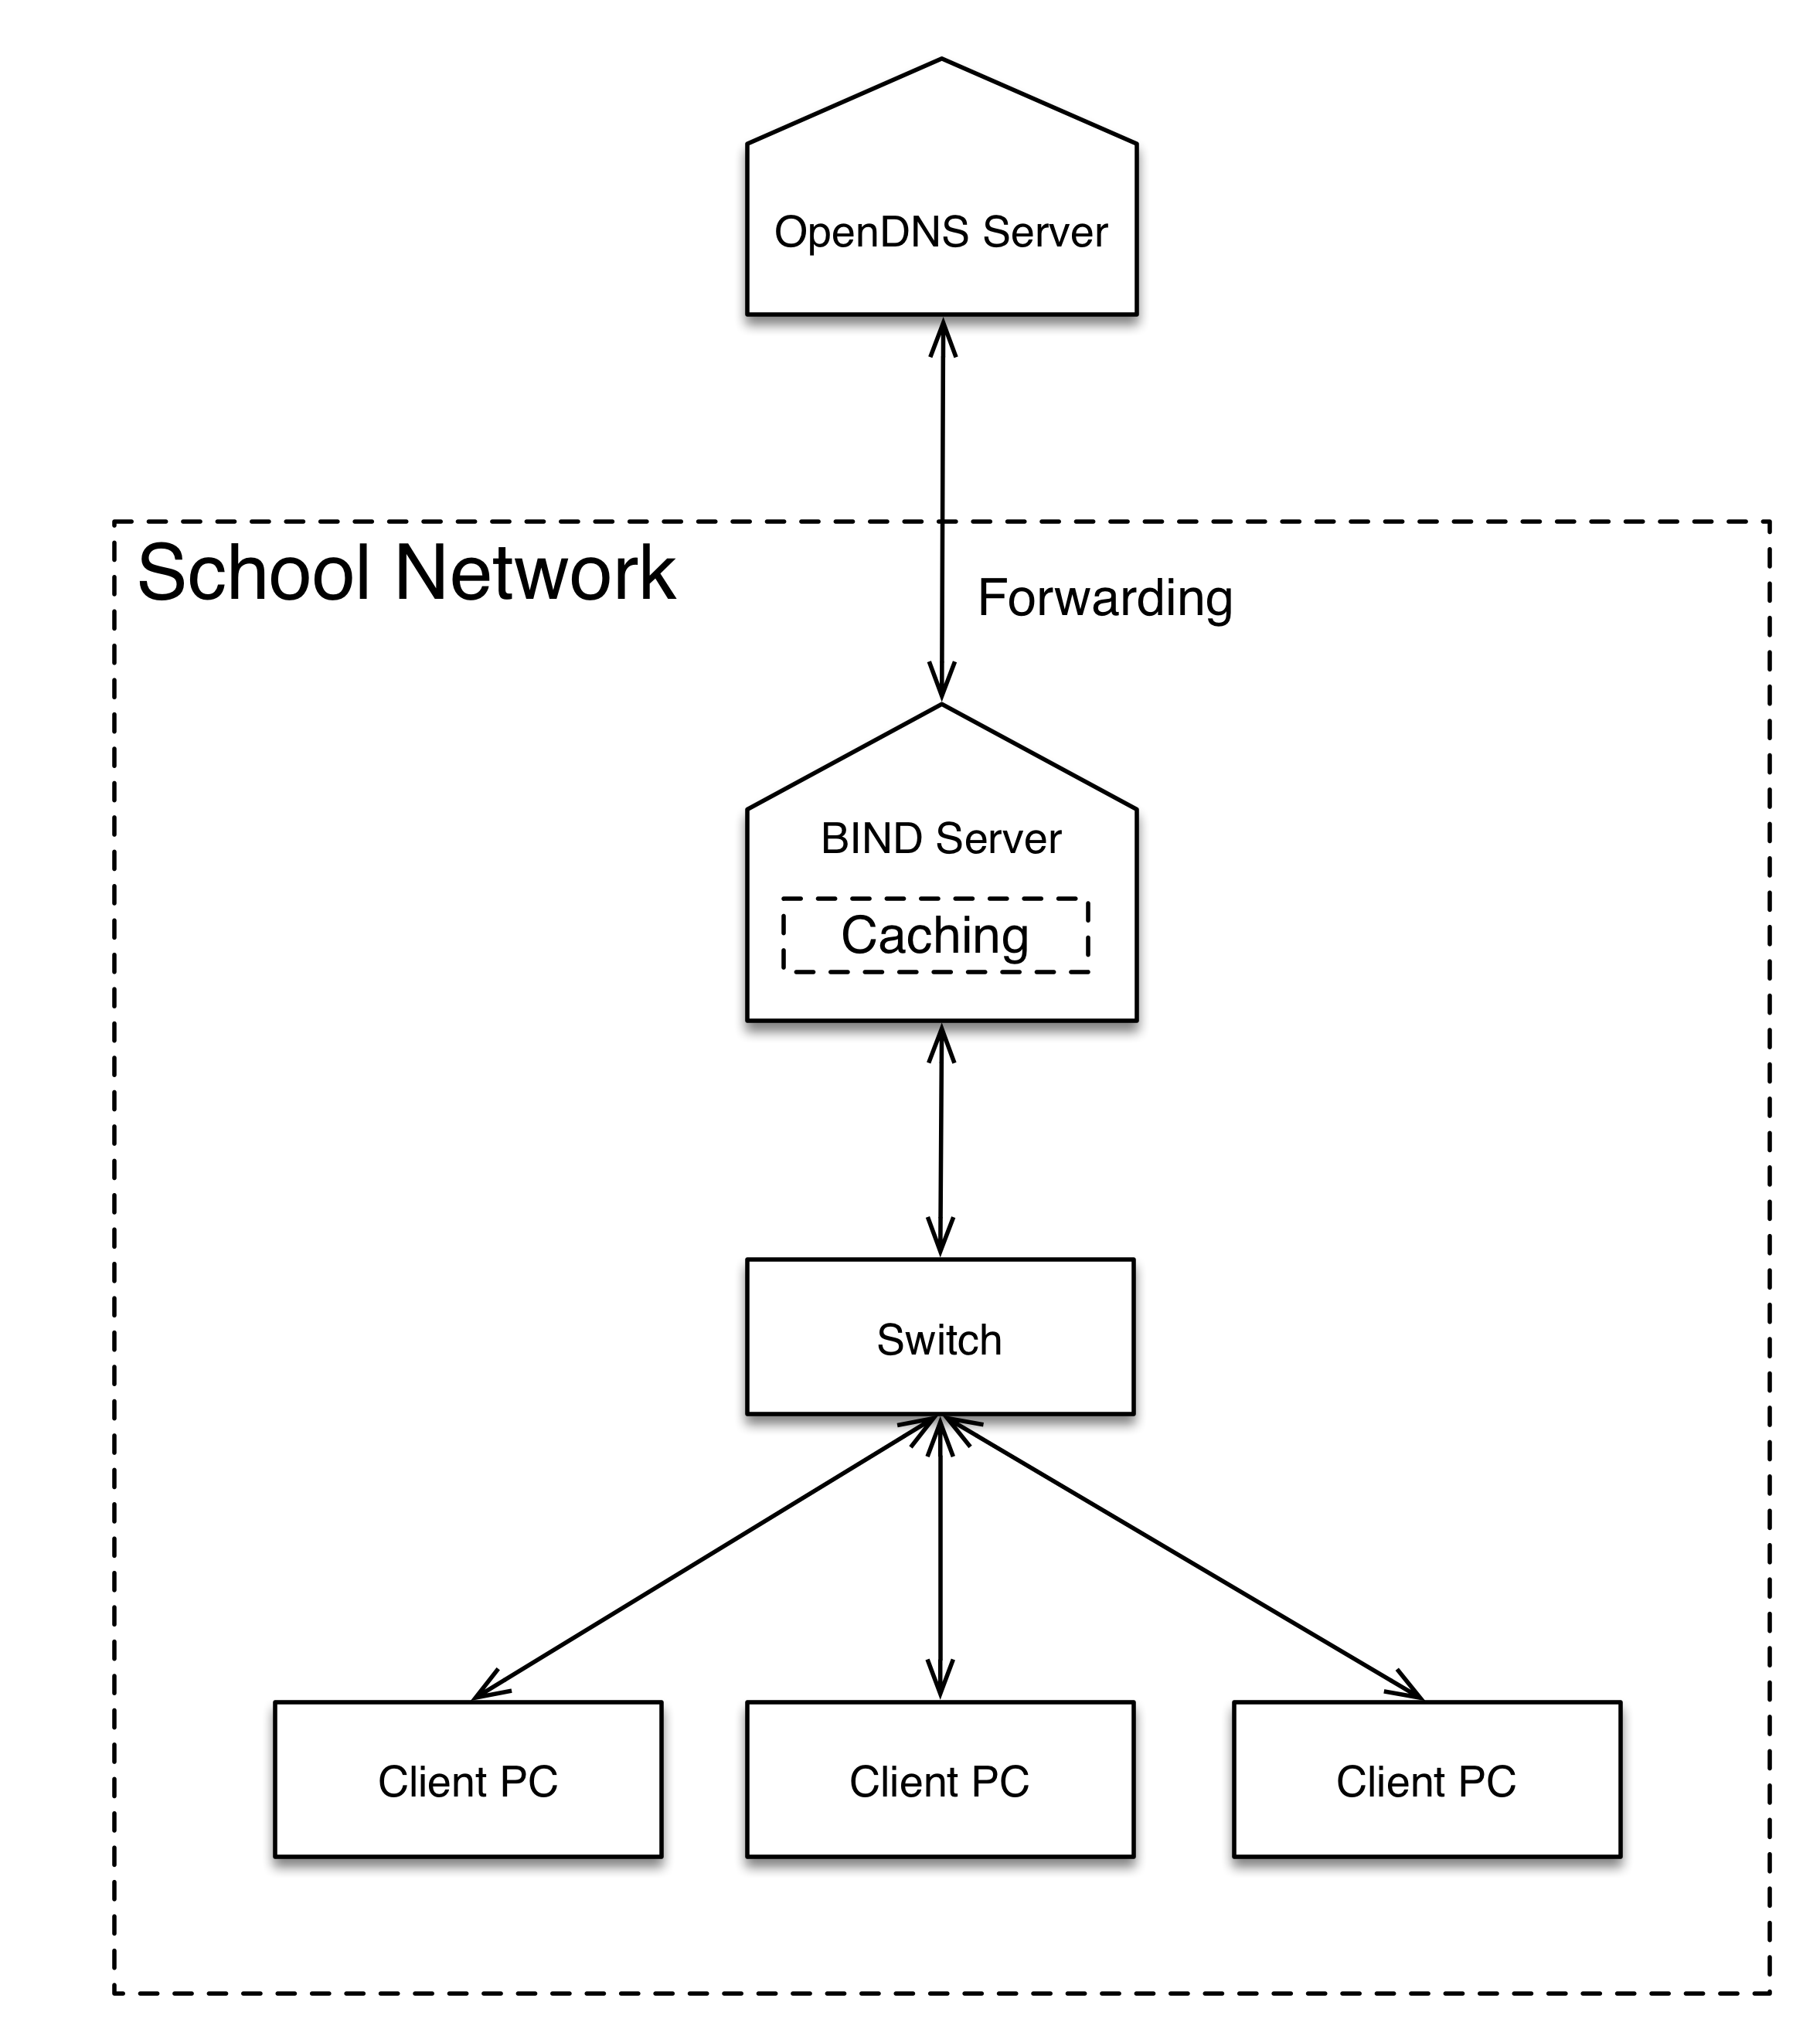
\includegraphics[width=90mm]{img/prototype_network_diagram.png}
\caption{School network with BIND server.}
\label{prototype_network_diagram}
\end{figure}

\section{Implementation}
To host the DNS, BIND is used. A general guide to setup BIND is found in section \ref{sec:binddnsserver}.

\subsection{Caching}
Since the caching name server functionality is activated by default, this feature needs no further setup.

\subsection{Forwarding}
The only thing to change in the forwarding setup process is changing the use of Googles DNS to OpenDNS instead. In \emph{/etc/bind/named.conf.options} OpenDNS' address is inserted like this:

\texttt{//Forwarding to OpenDNS} \\
\texttt{forwarders \{208.67.222.222; 208.67.220.220;\};}

\section{Test}
\subsection{Caching}
To test this functionality a previously unvisited site is checked with dig, twice. 

\begin{figure}[ht!]
\centering
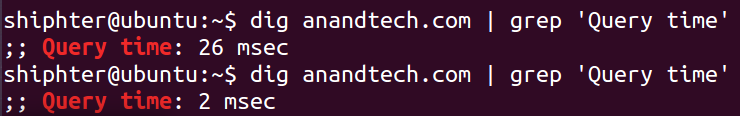
\includegraphics[width=90mm]{img/prototype_caching_test.png}
\caption{Prototype testing of Caching Name Server.}
\label{prototype_caching_test}
\end{figure}

The drastic performance improvement indicates that caching functionality is fully functional. 

\subsection{Forwarding}
